\documentclass[1pt]{article}
\usepackage[margin=1in]{geometry}
\usepackage{graphicx}
\usepackage{listings}
\usepackage{enumitem}
\graphicspath{{/Users/diesel/Desktop/}}
\usepackage{tabu}

\title{ Cost of Computing in the Cloud}
\author{Saptarshi Chatterjee \\
\texttt{MS, Illinois Institute of Technology }\\
}

\begin{document}
\maketitle

\texttt{Please refer to "costcalc.xls" for formulas, calculations and references}\\

\section{Configuration 1: Hadoop/Spark Cluster with 32K-cores, 256TB memory, 50PB HDD, and 10Gb/s Ethernet
Fat-Tree network (each VM should be equivalent to the d2.8xlarge instance); in addition to the compute
resources, a 100PB distributed storage shared across the entire cloud should be procured, with enough
capacity for 100GB/sec throughput (for pricing comparison, see S3)}

\setlength{\parskip}{1.2em}
\setlength{\parindent}{0em}

\emph{Cost of Private Cloud }\\
\\
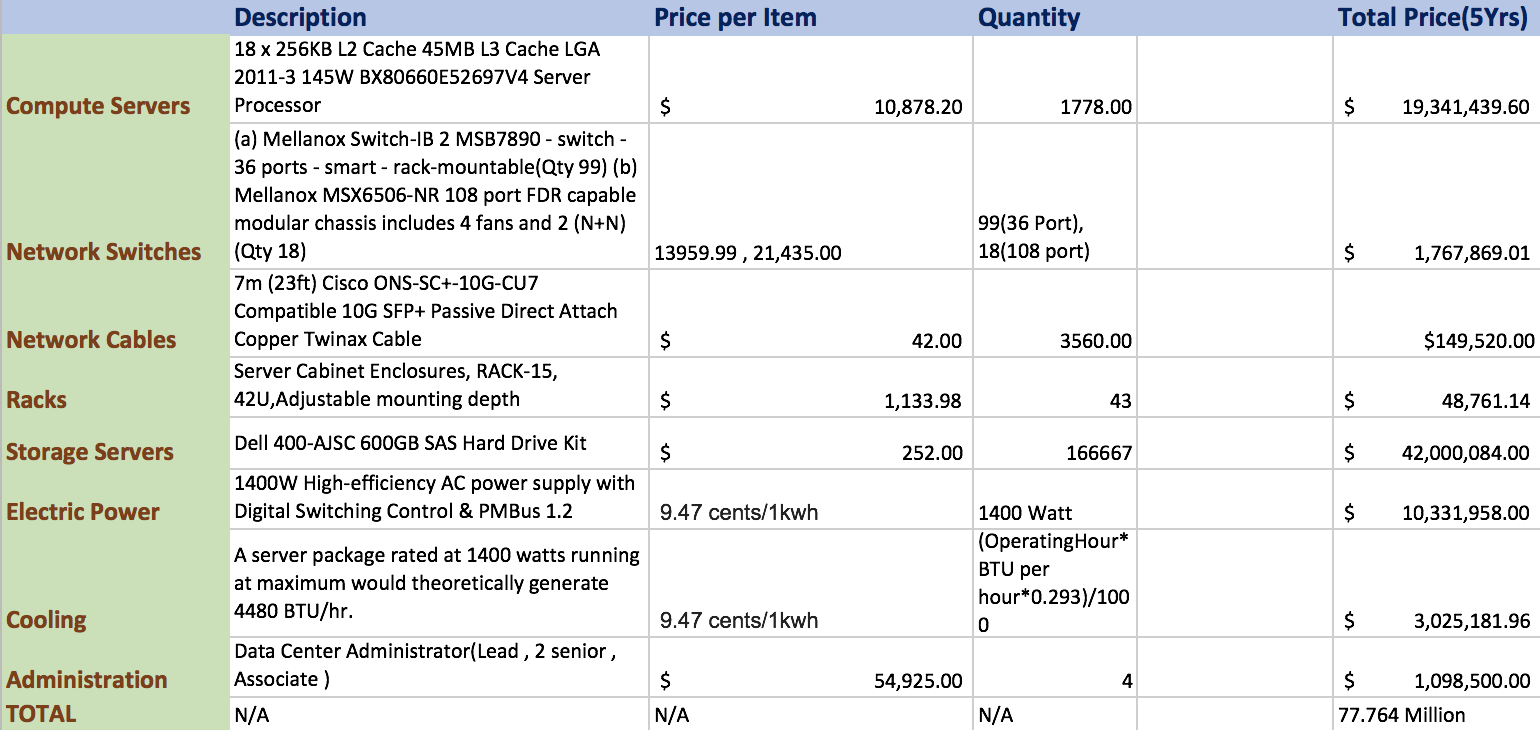
\includegraphics[scale=.6]{config1Pr}\\

 \clearpage
\emph{Cost of Public Cloud }\\
\\
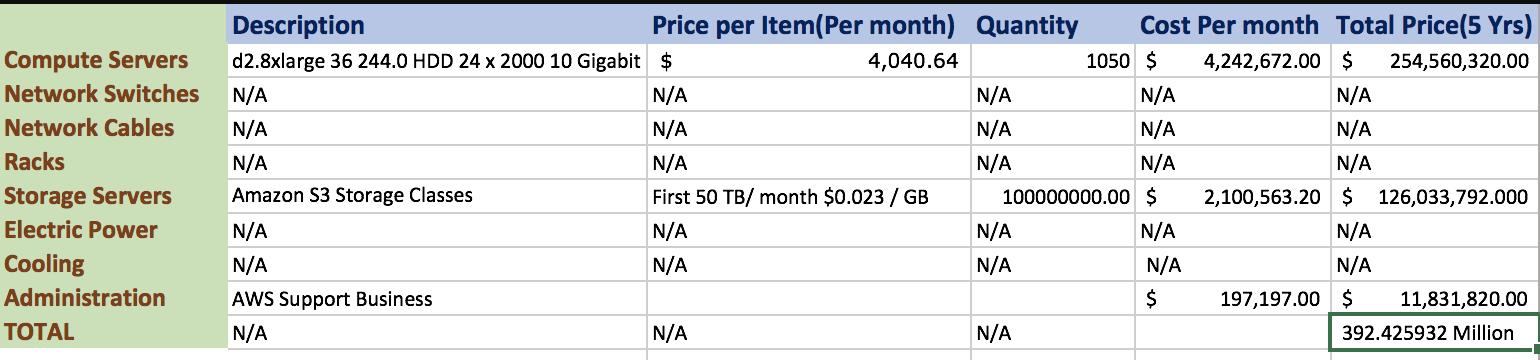
\includegraphics[scale=.6]{config1Pu}\\

\emph{AWS cost }\\
\\
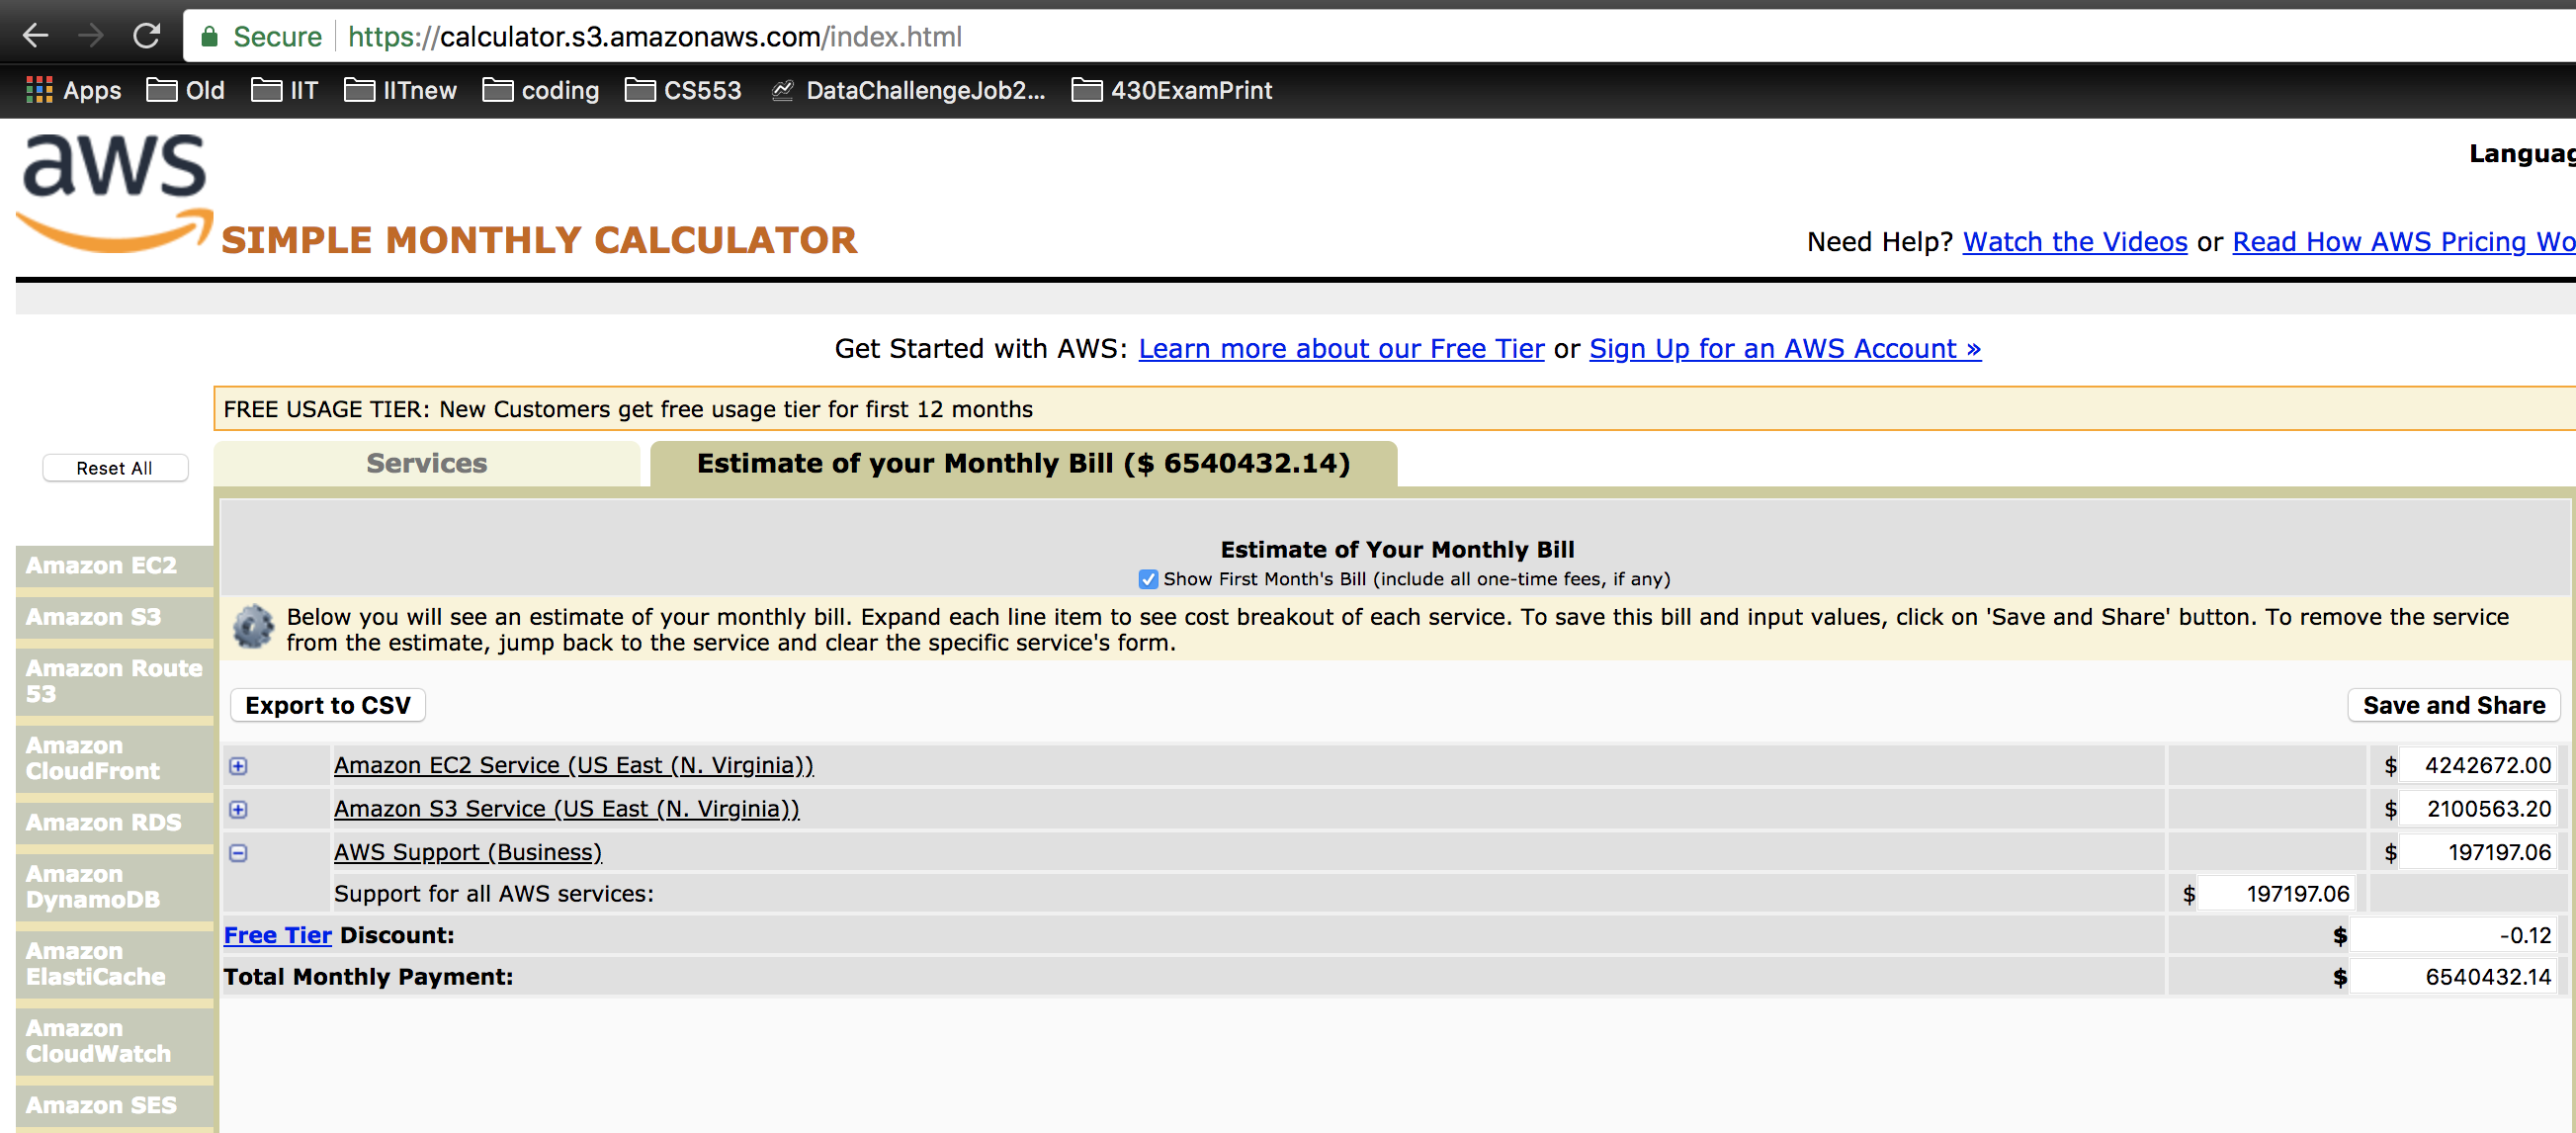
\includegraphics[scale=.3]{config1Aws}\\

\emph{CPU, Memory and Storage config }\\
\\
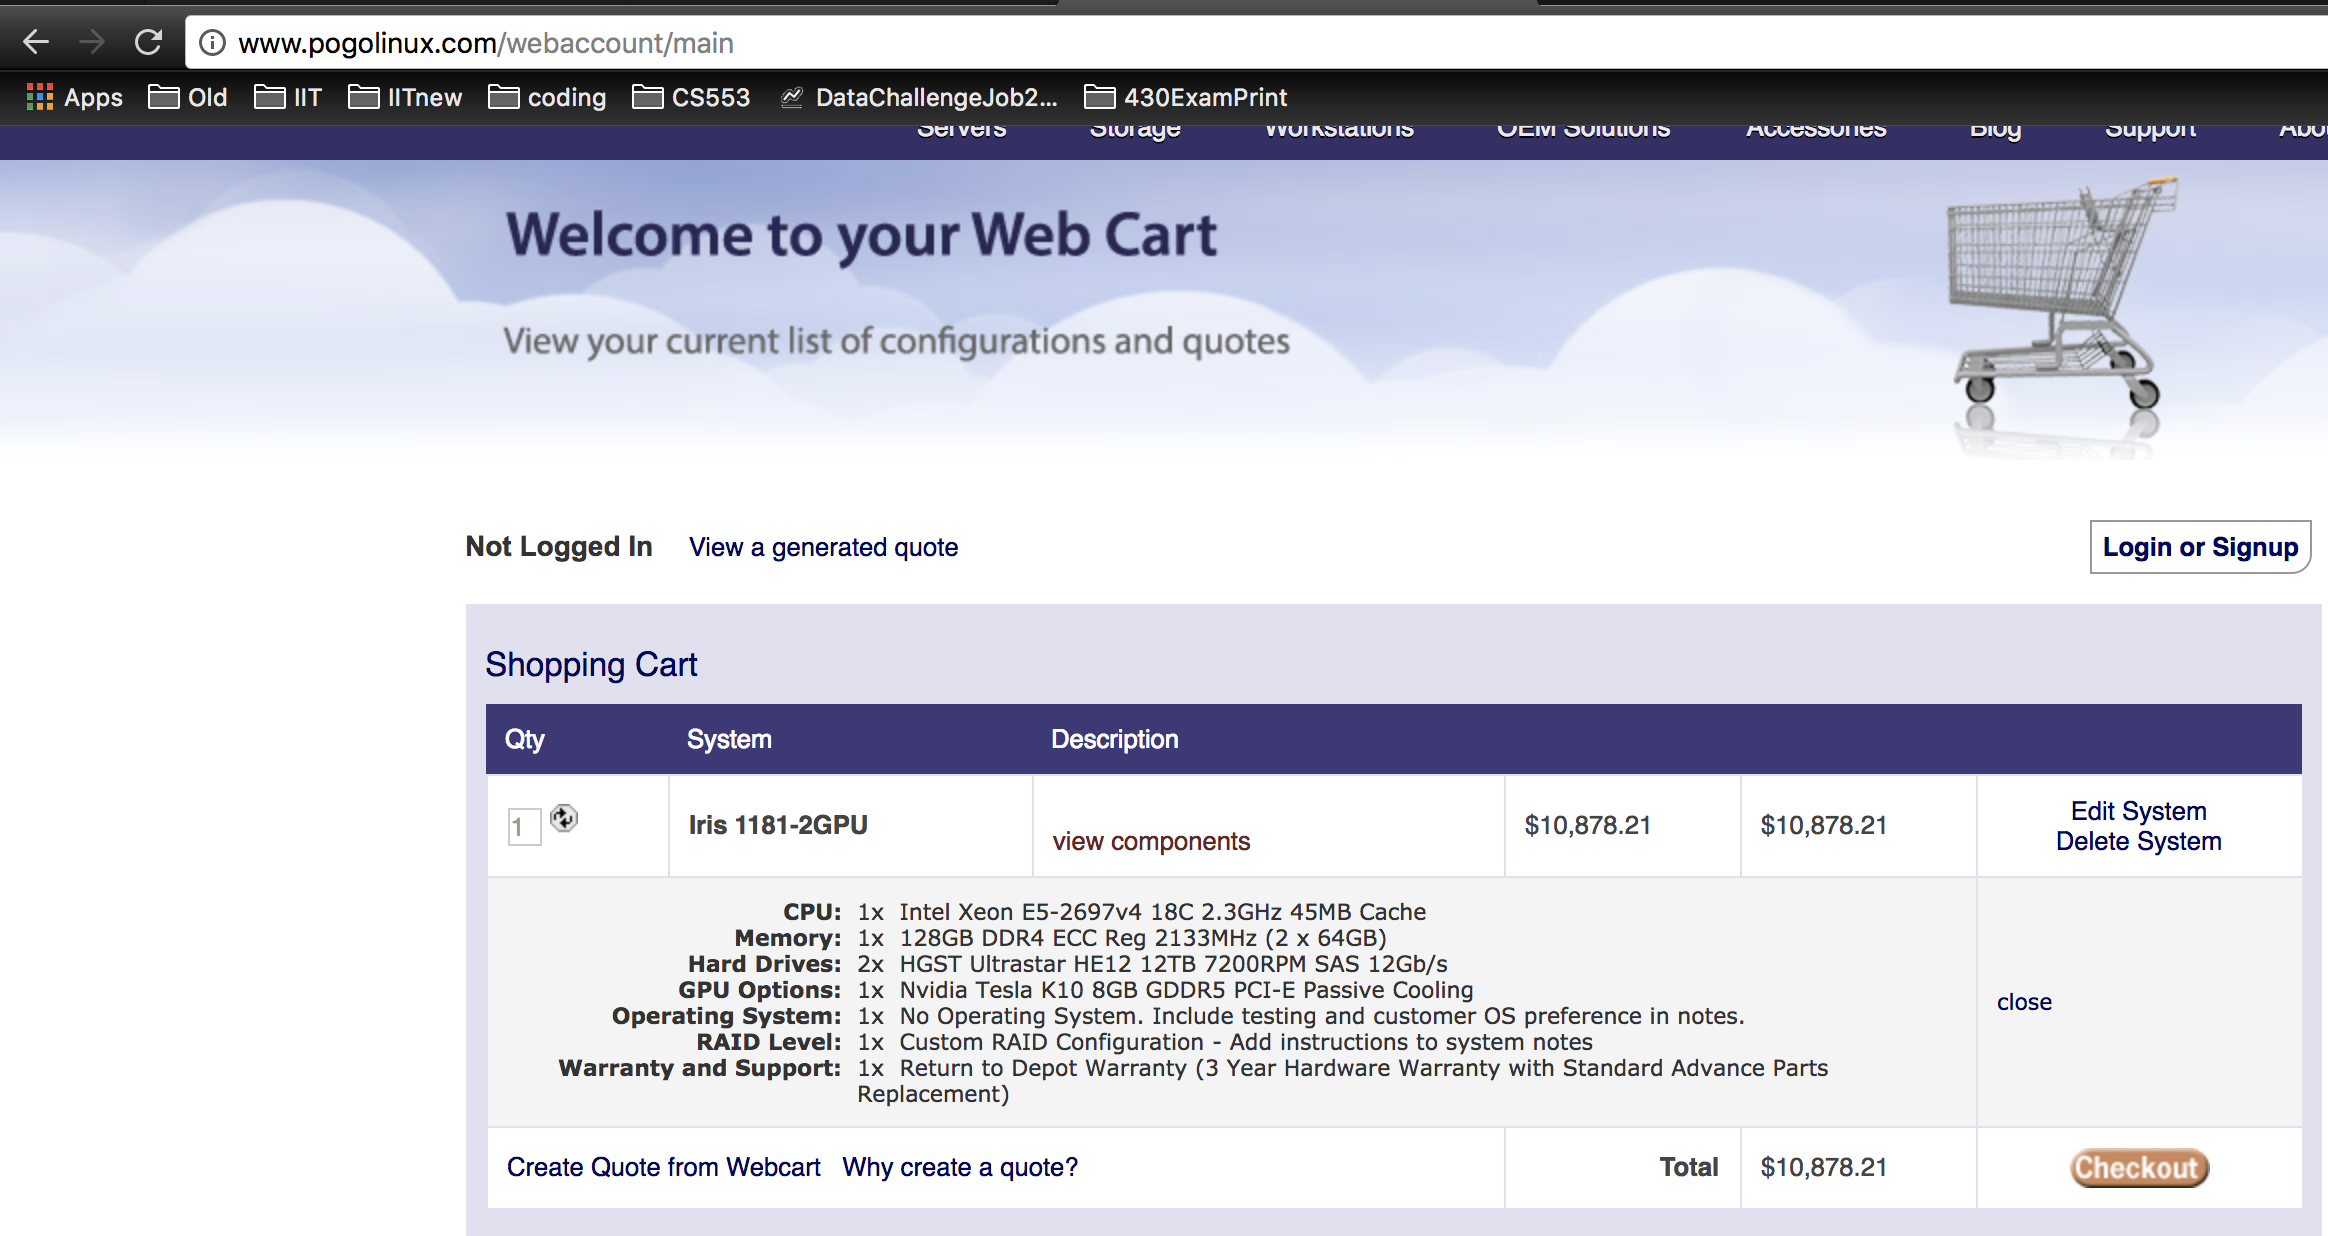
\includegraphics[scale=.3]{cpuConfig1}\\

\emph{Fat-Tree network Infiniband}\\
\\
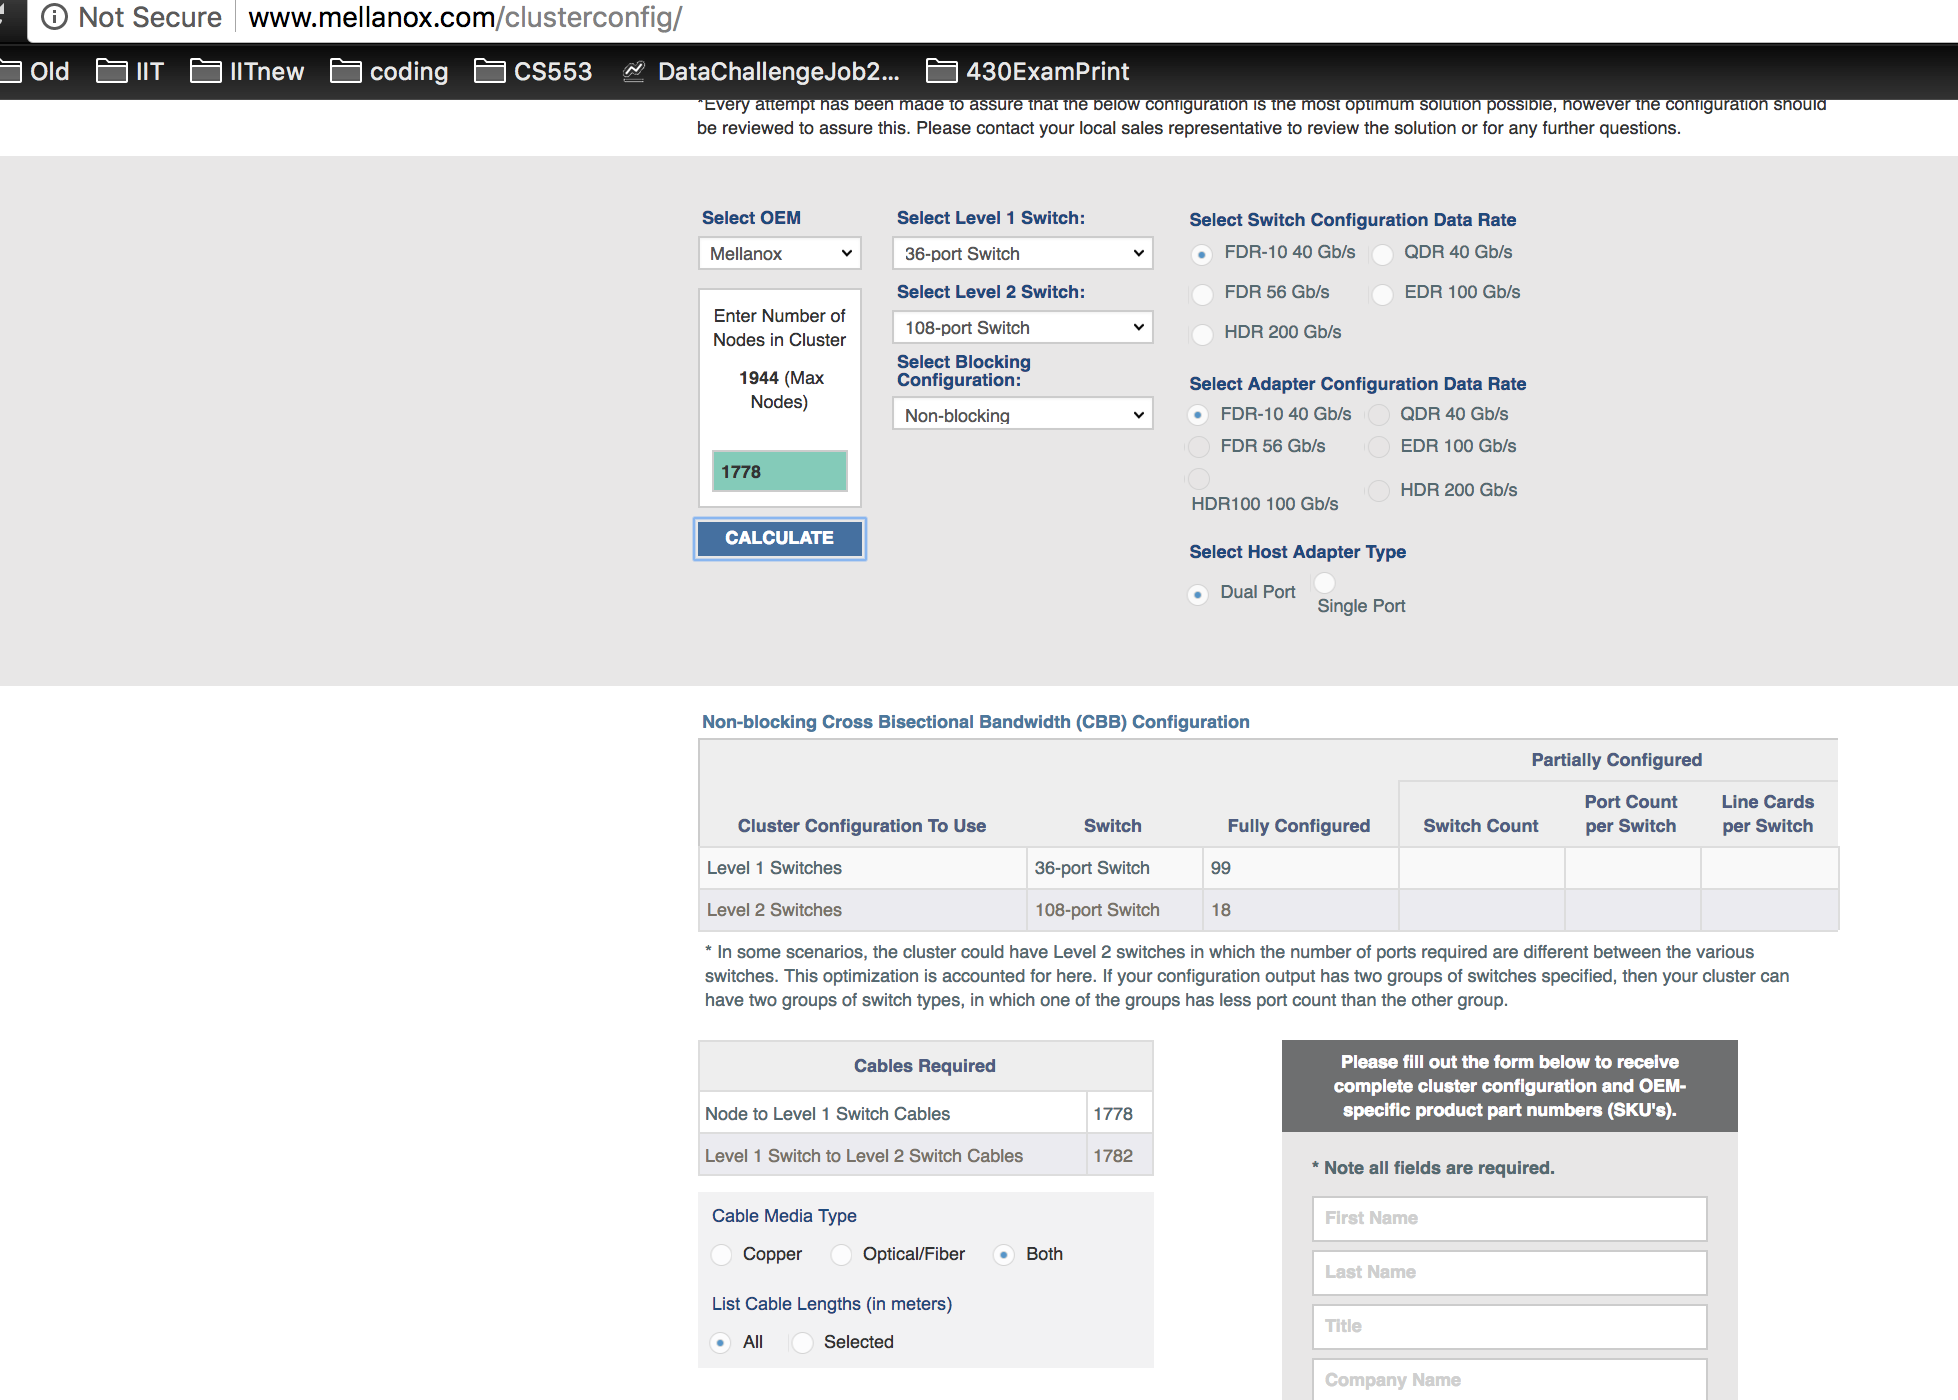
\includegraphics[scale=.5]{switchConfig1}\\

\emph{Power usage}\\
\\
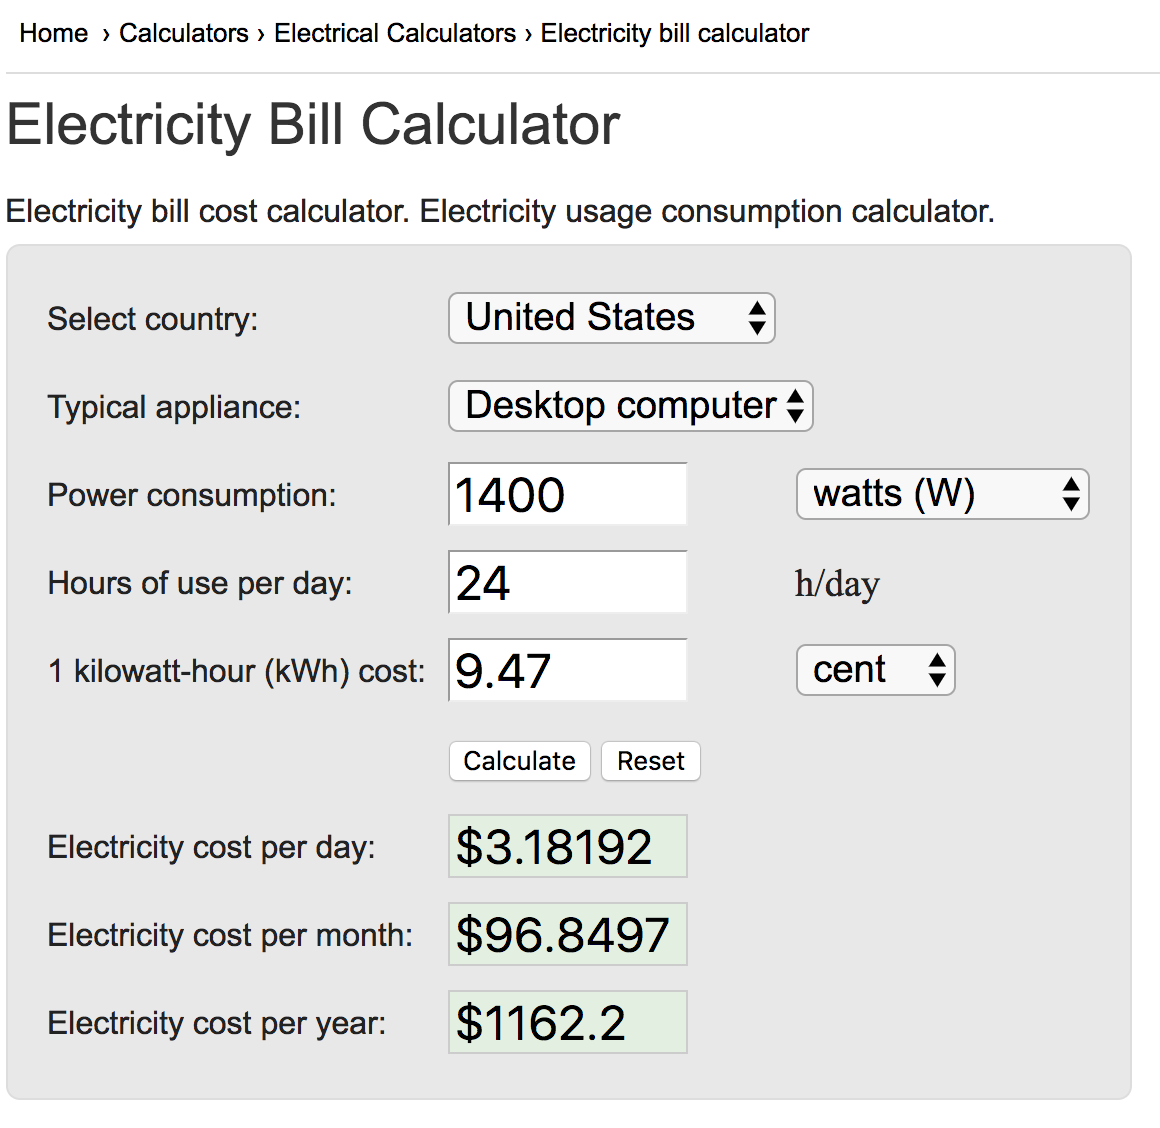
\includegraphics[scale=.3]{electricity1}\\


\section{Configuration 2: Support 1 million virtual machines (VM) where each VM requires 2-core, 15GB RAM, 32GB
SSD storage, and 1Gb/s Fat-Tree network (each VM should be equivalent to the r3.large instances); in
addition to the compute resources, a 10PB distributed storage shared across the entire cloud should be
procured, with enough capacity for 10GB/sec throughput (for pricing comparison, see S3)}

\setlength{\parskip}{1.2em}
\setlength{\parindent}{0em}

\emph{Cost of Private Cloud }\\
\\
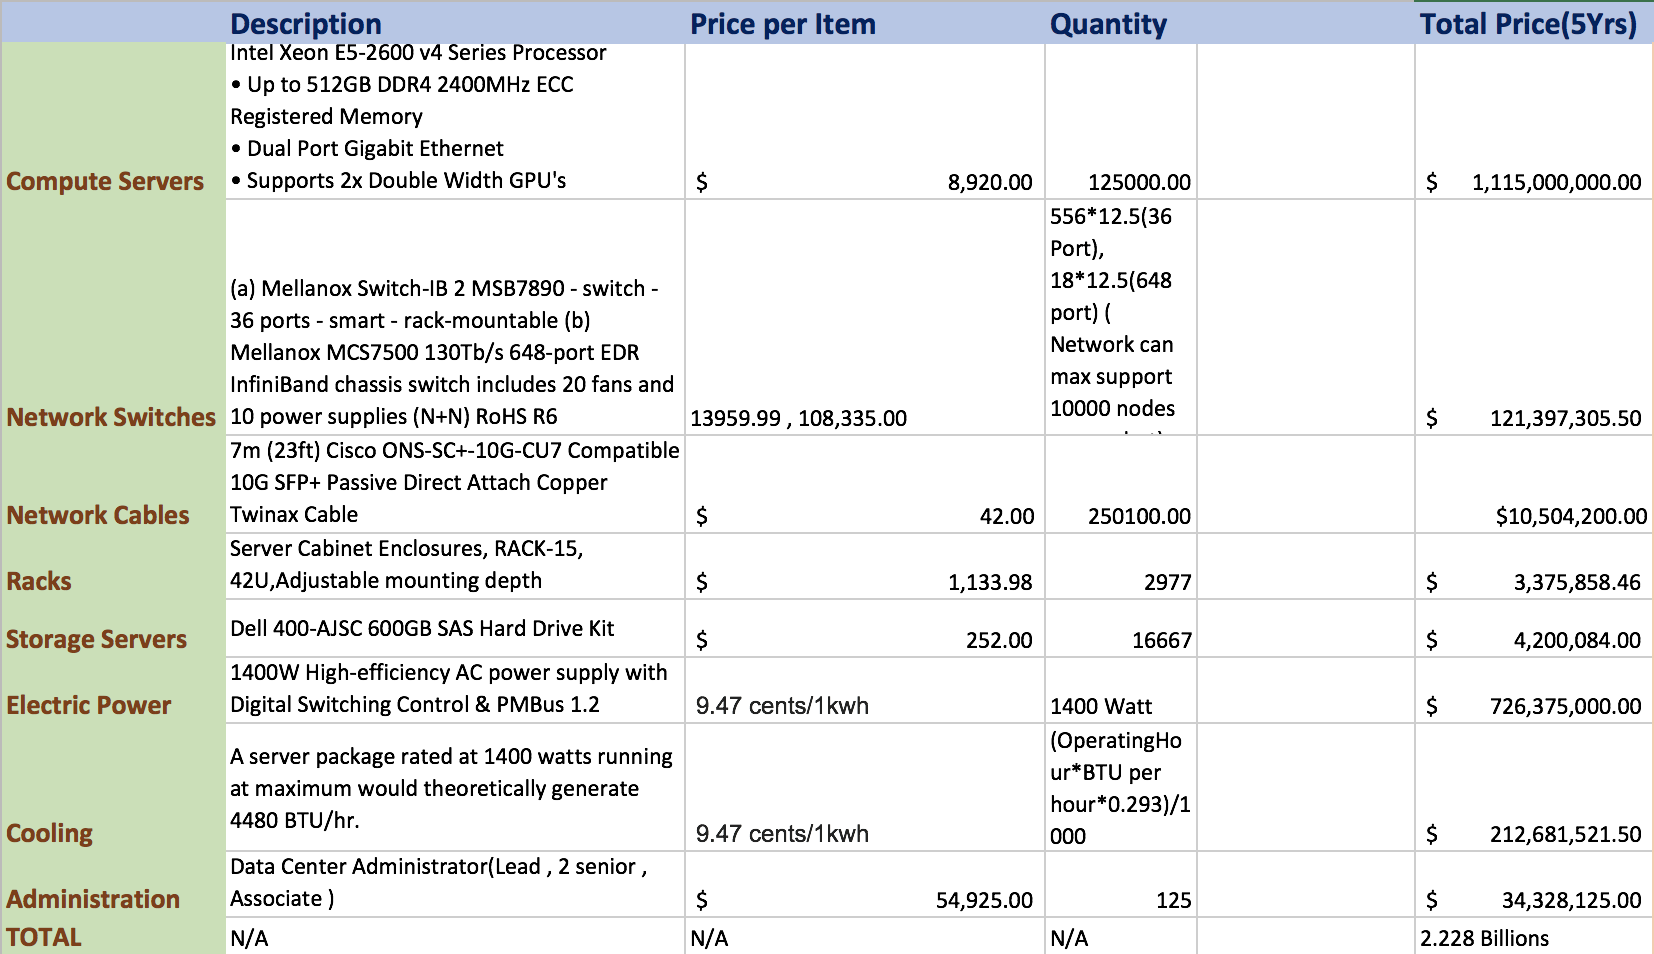
\includegraphics[scale=.6]{config2Pr}\\

\emph{Cost of Public Cloud }\\
\\
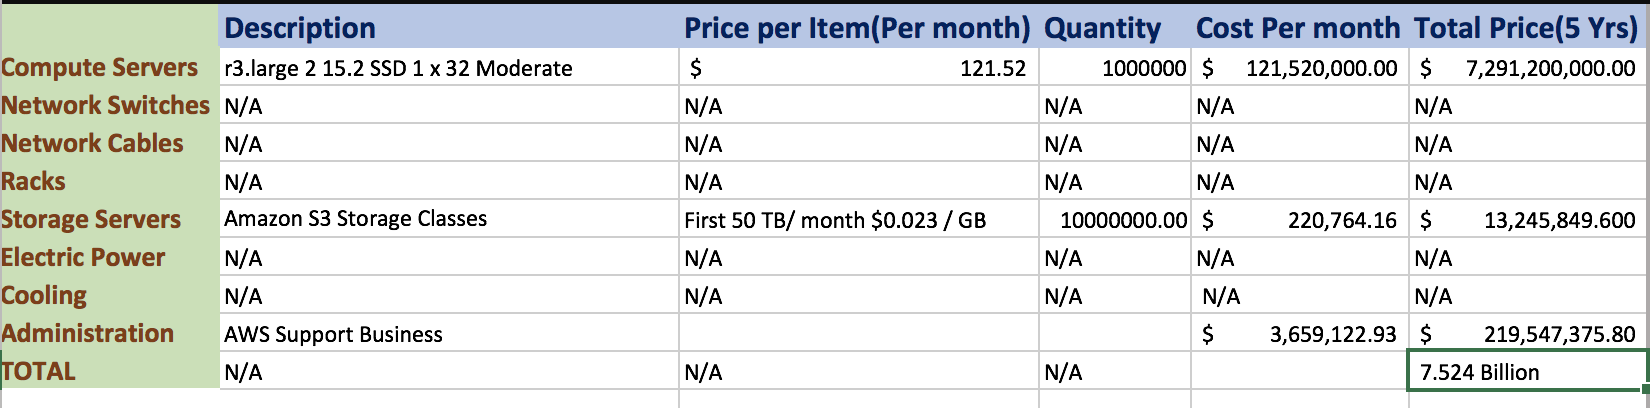
\includegraphics[scale=.6]{config2Pu}\\

\emph{AWS cost }\\
\\
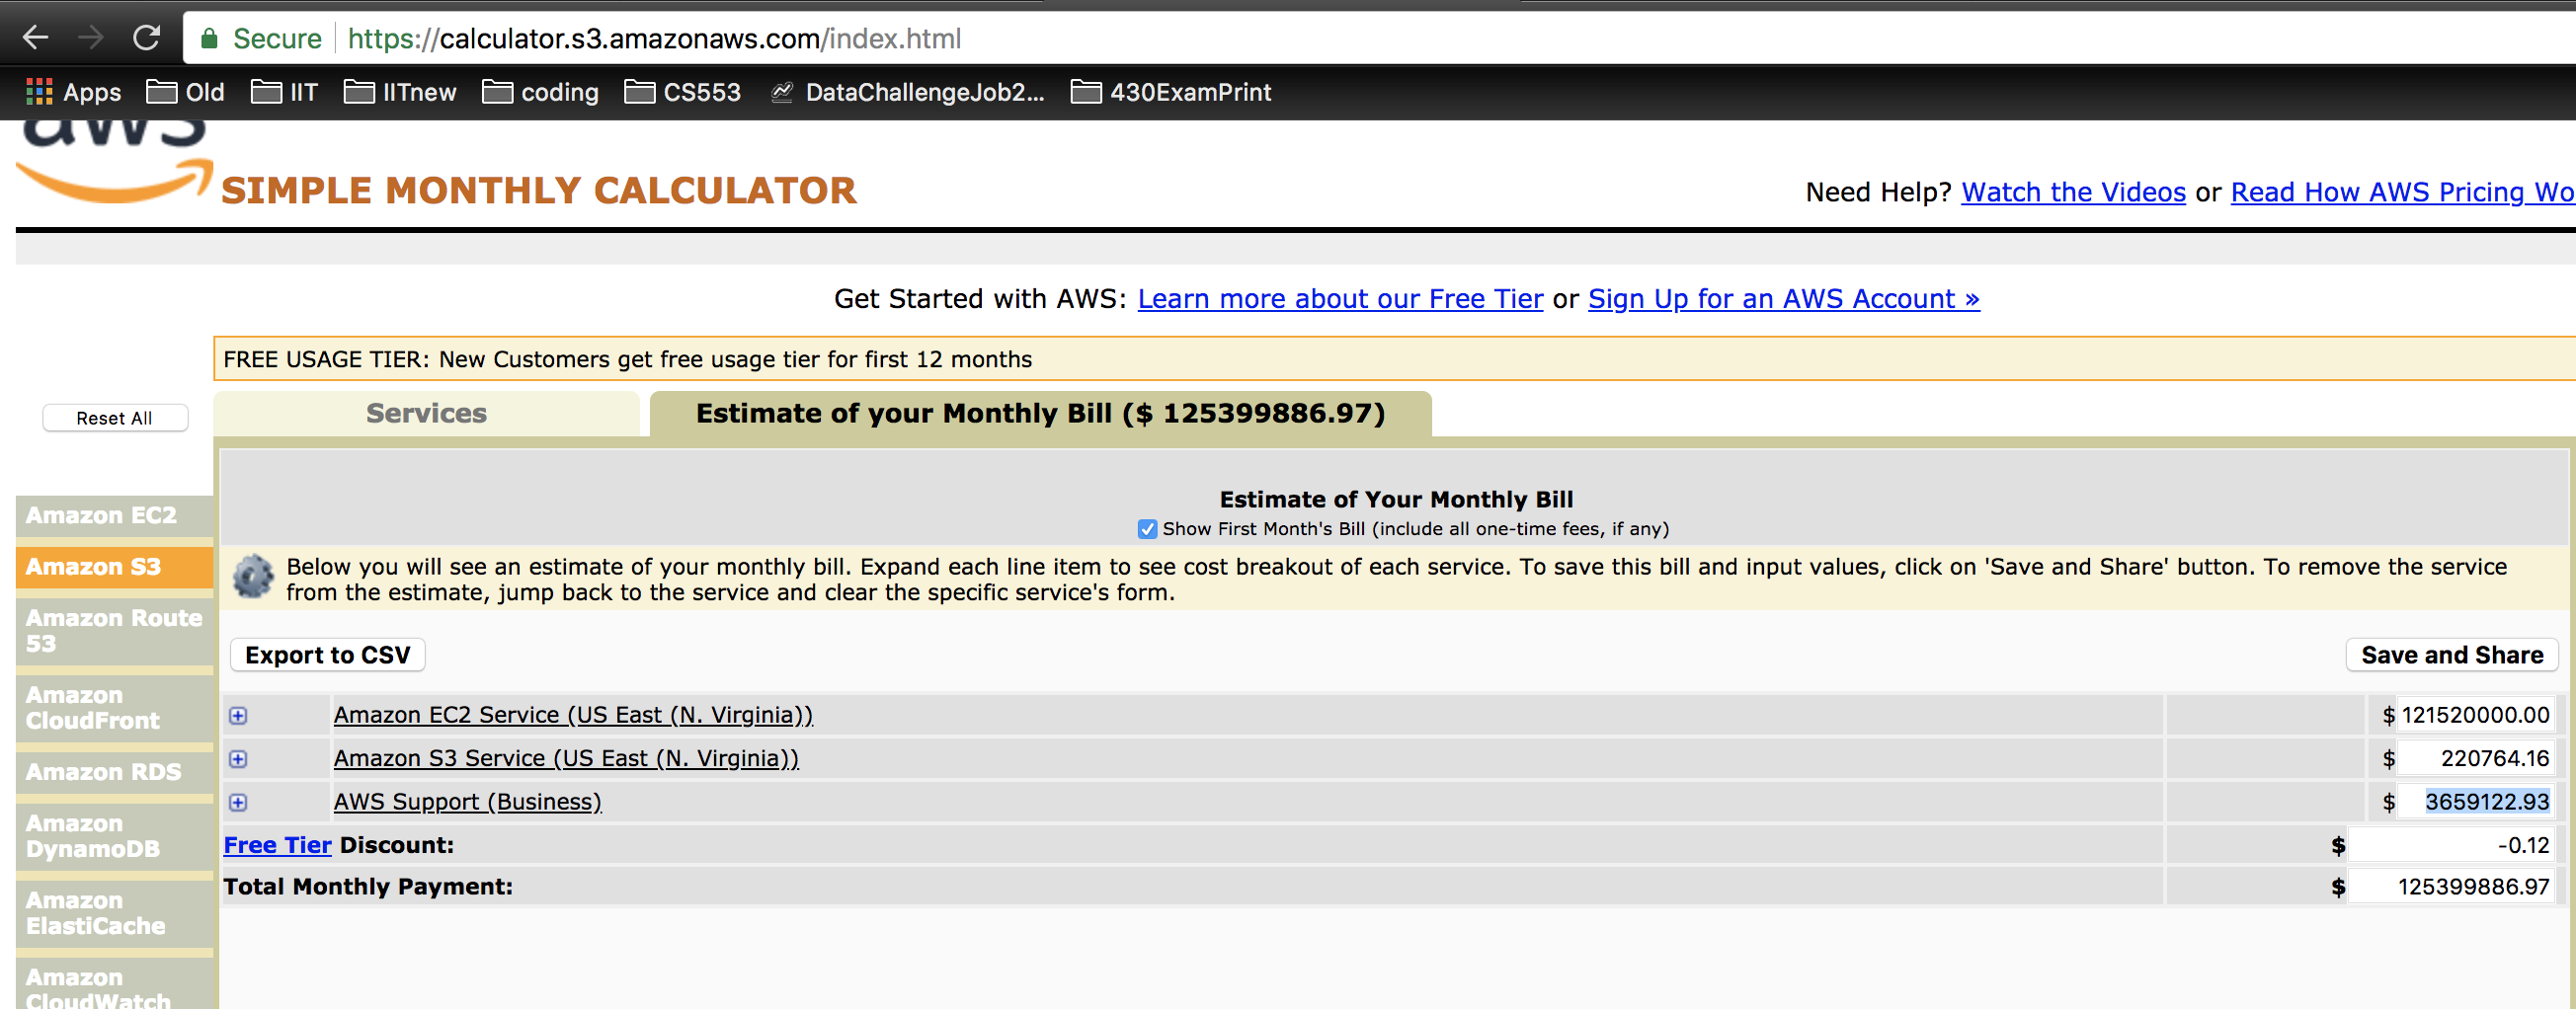
\includegraphics[scale=.3]{config2Aws}\\

\emph{CPU, Memory and Storage config }\\
\\
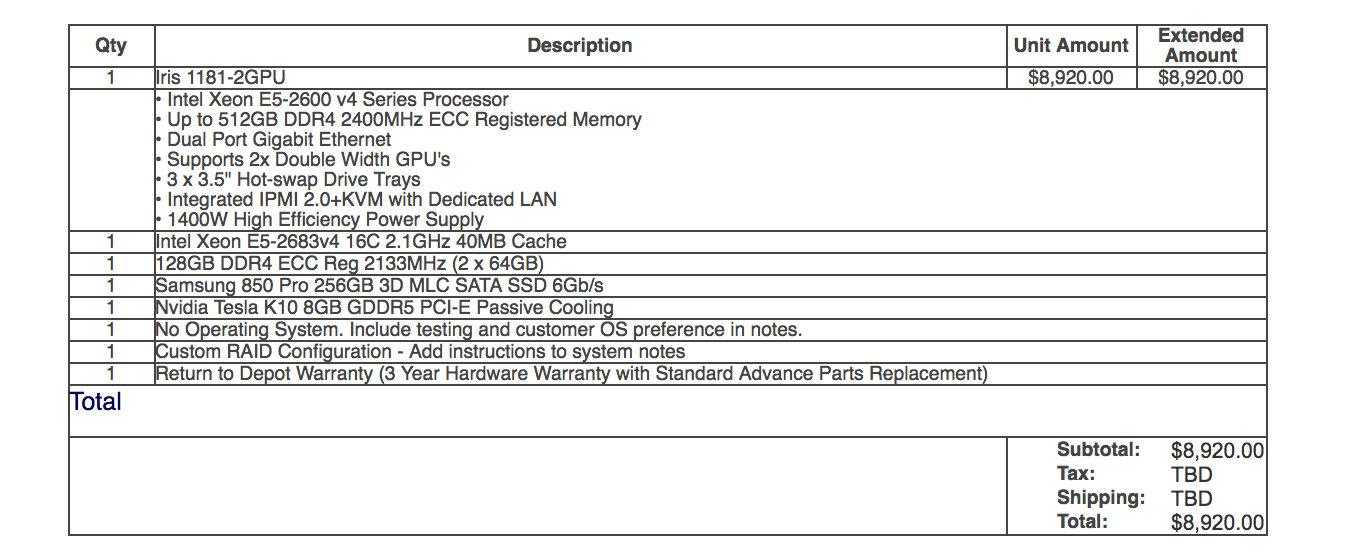
\includegraphics[scale=.6]{cpuConfig2}\\

\emph{Fat-Tree network Infiniband}\\
\\
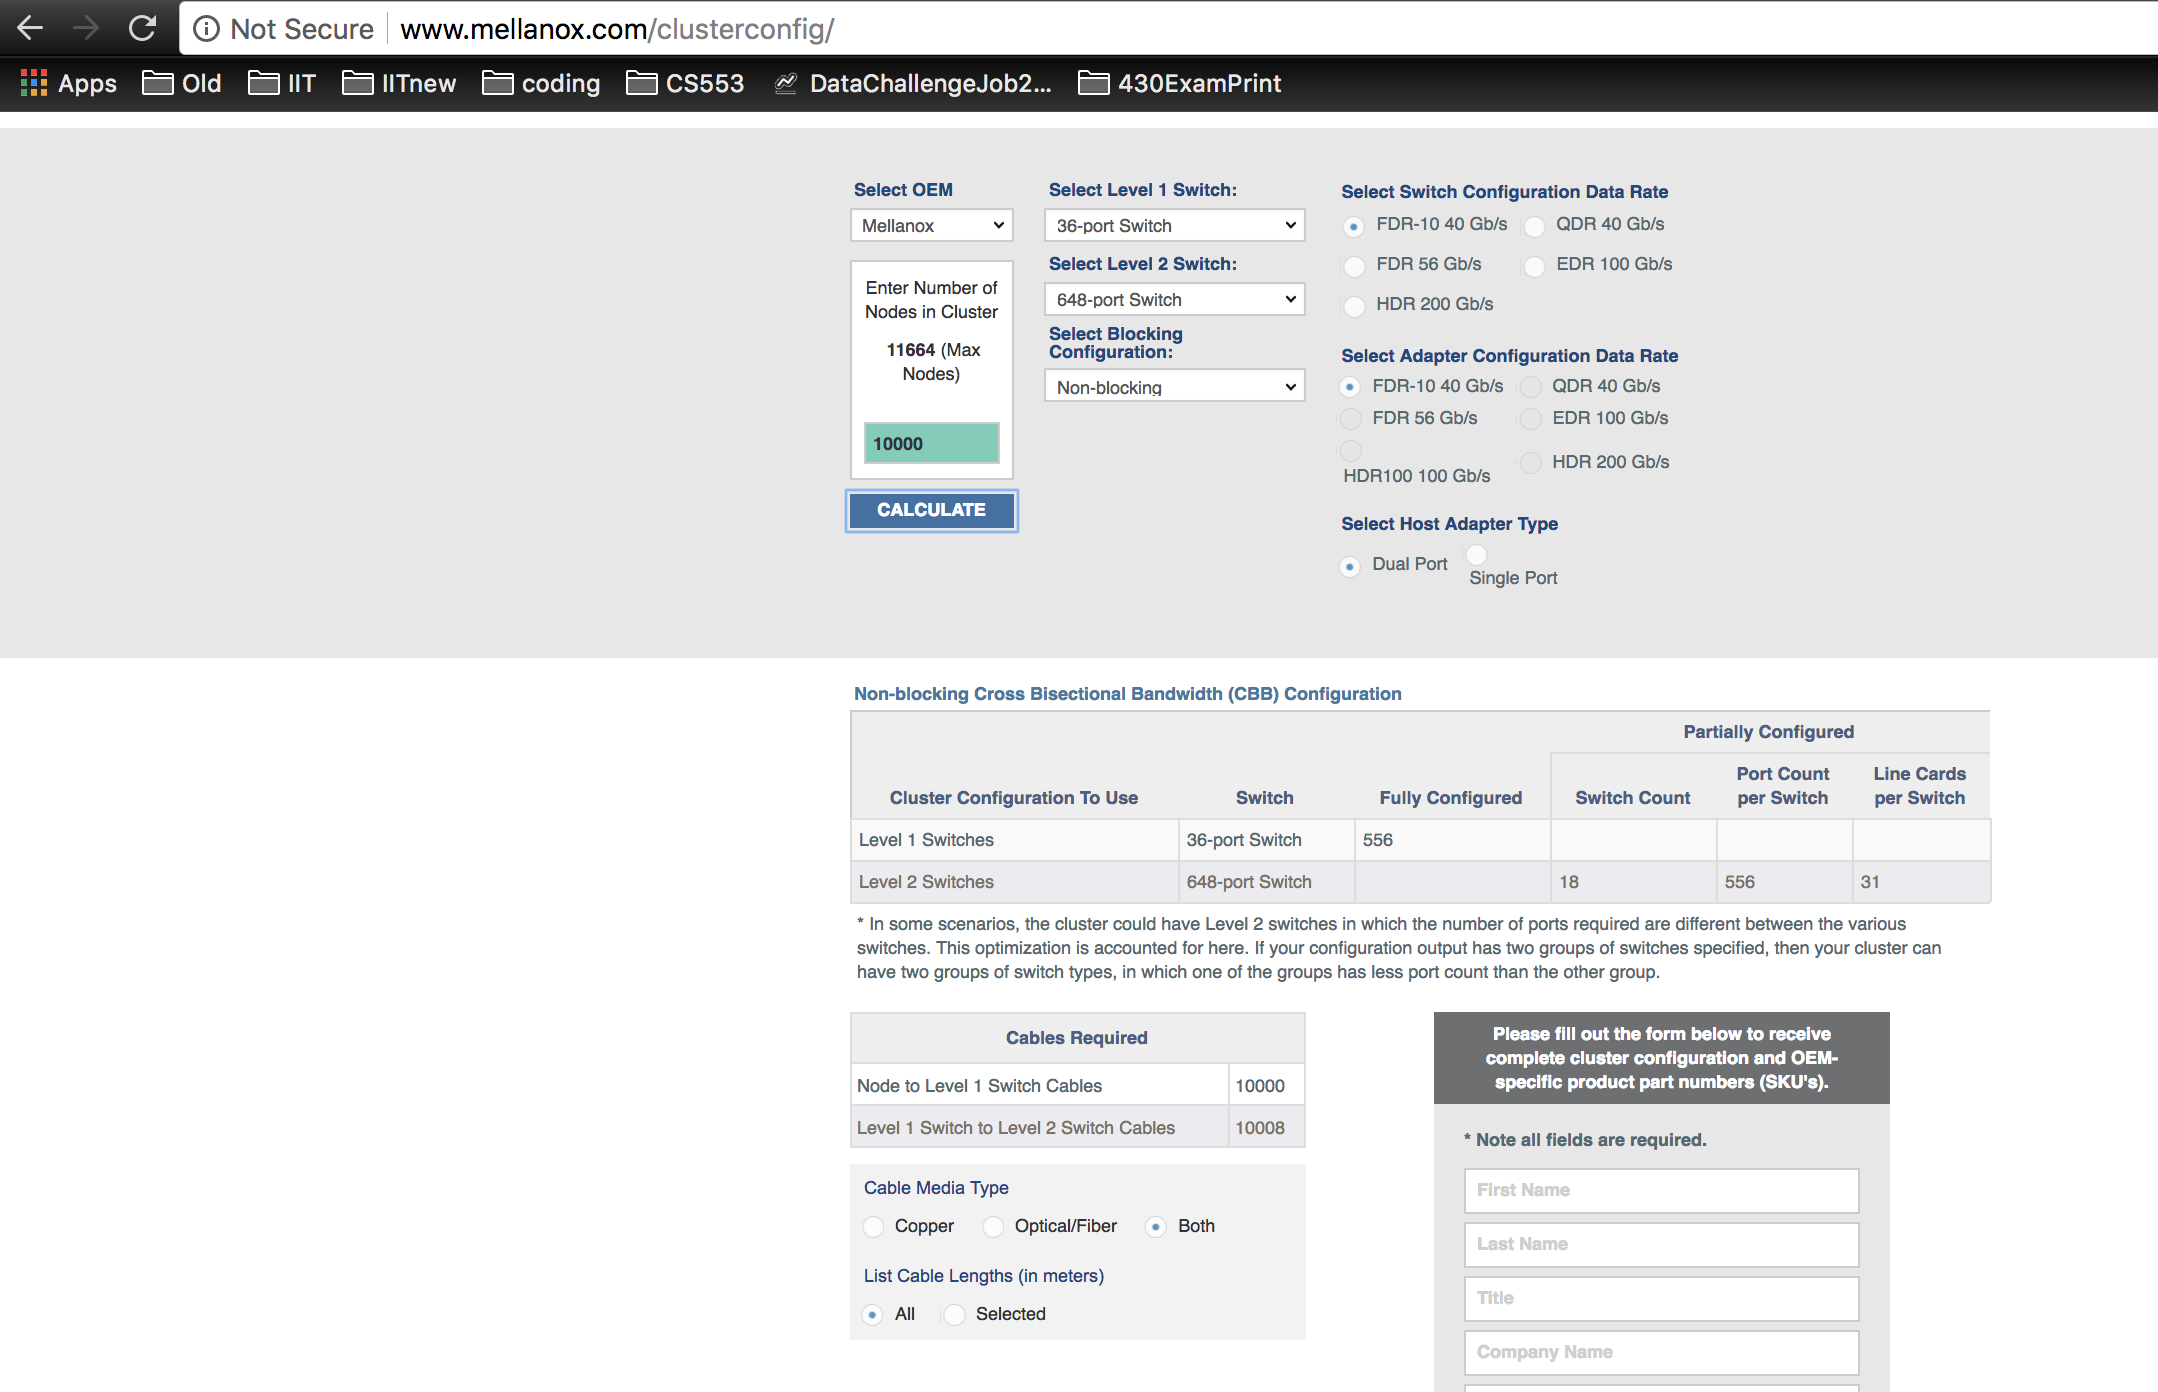
\includegraphics[scale=.4]{switchConfig2}\\

\emph{Power usage}\\
\\
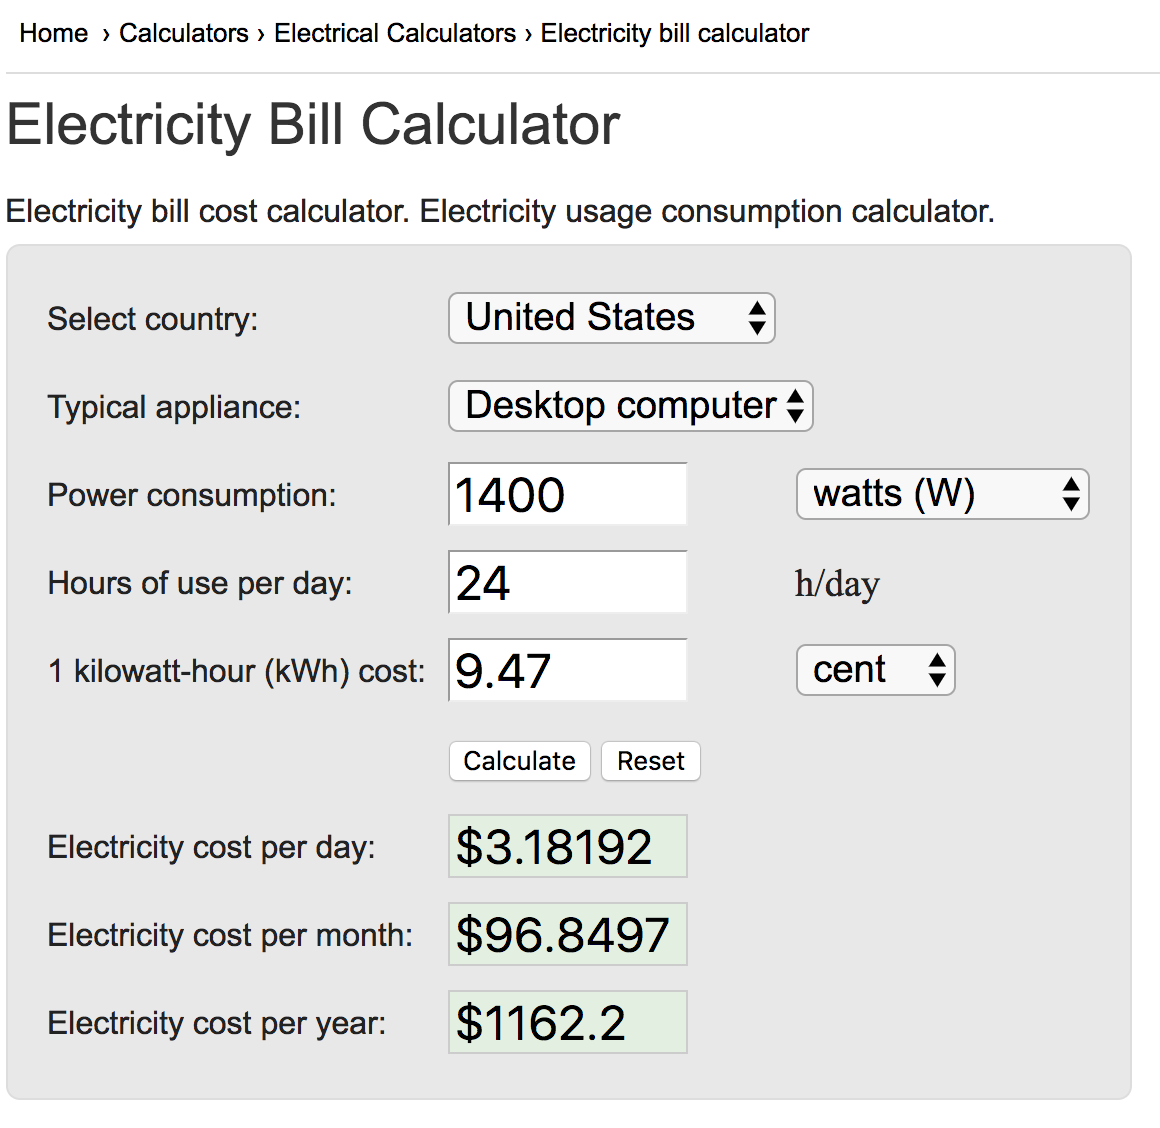
\includegraphics[scale=.3]{electricity1}\\

\section{Configuration 3: Support deep learning with 1 exaflop of mixed precision performance (hint: each VM
should be equivalent to p3.16xlarge instances; you will want to use the NVIDIA V100 GPUs (8 GPUs per
node), and allocate 8-cores per GPU (64-cores per node) with 8GB of memory per core (512GB per node);
the network to use is at least 10Gb/s per GPU (100Gb/s should work), and should be organized in a Fat-Tree
network; in addition to the compute resources, a 1PB distributed storage shared across the entire cloud
should be procured, with enough capacity for 10GB/sec throughput (for pricing comparison, see S3)}

\setlength{\parskip}{1.2em}
\setlength{\parindent}{0em}

\emph{Cost of Private Cloud }\\
\\
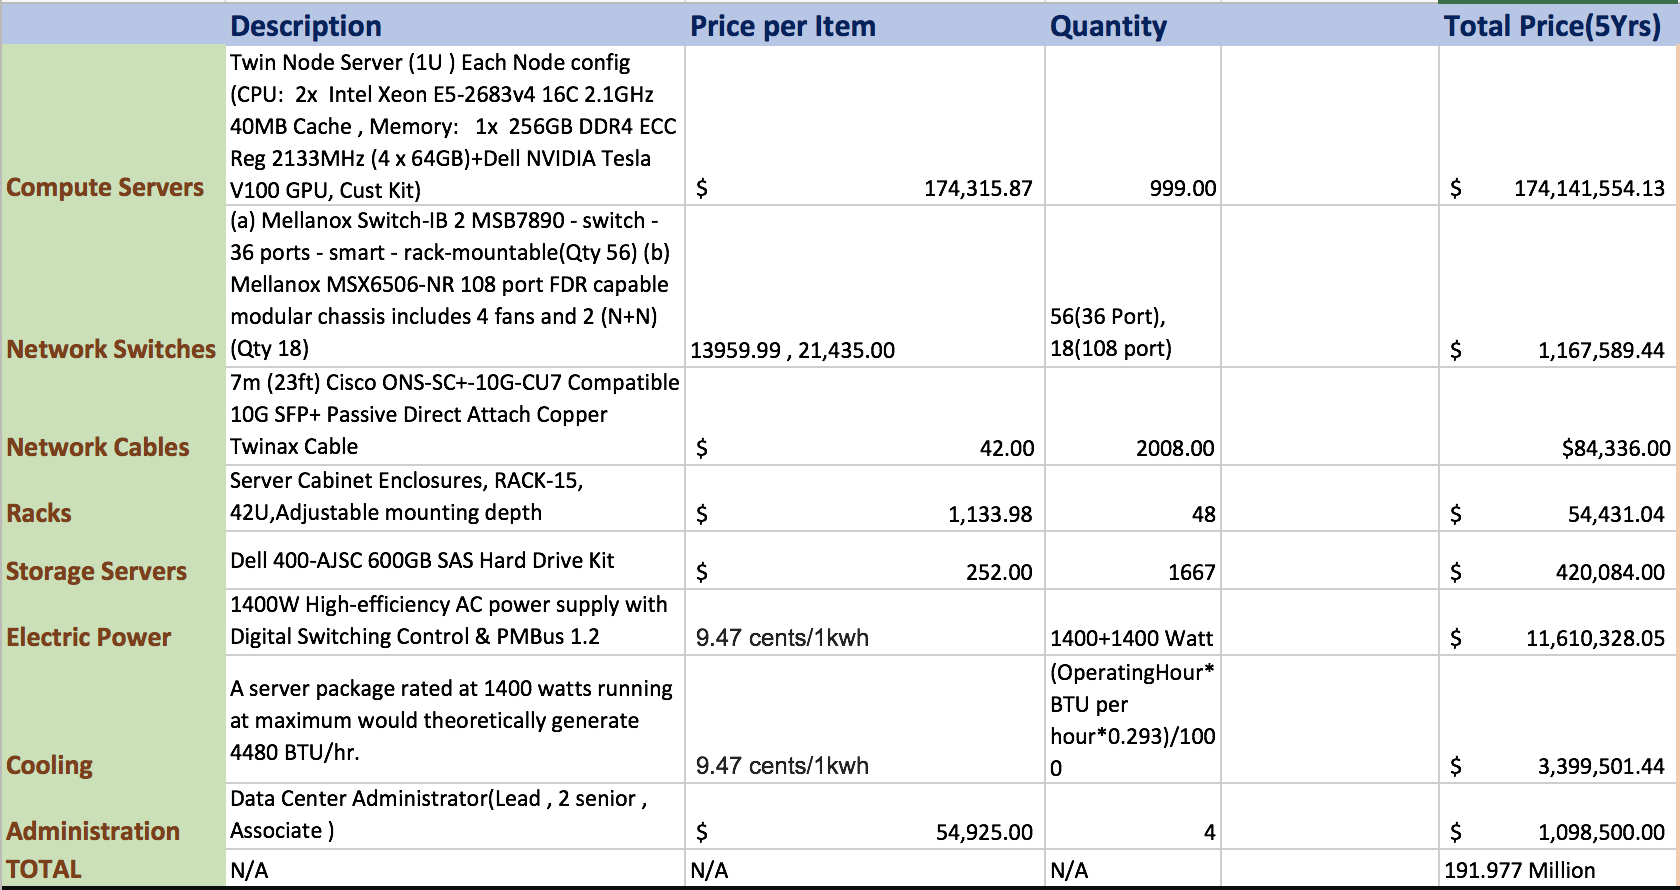
\includegraphics[scale=.6]{config3Pr}\\

\emph{Cost of Public Cloud }\\
\\
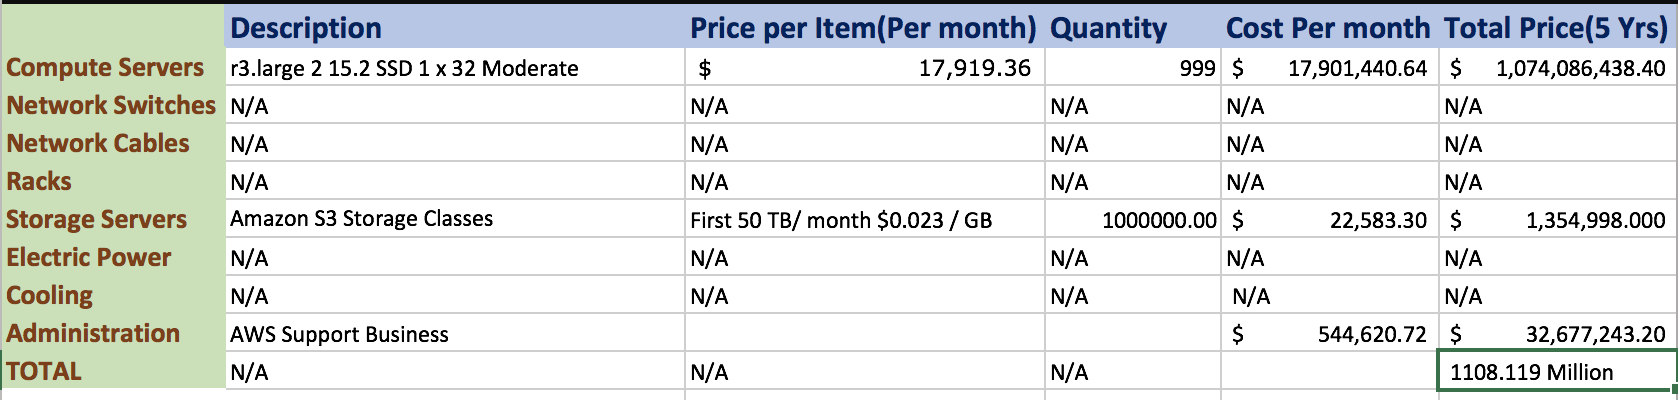
\includegraphics[scale=.6]{config3Pu}\\

\emph{CPU, Memory and Storage config }\\
\\
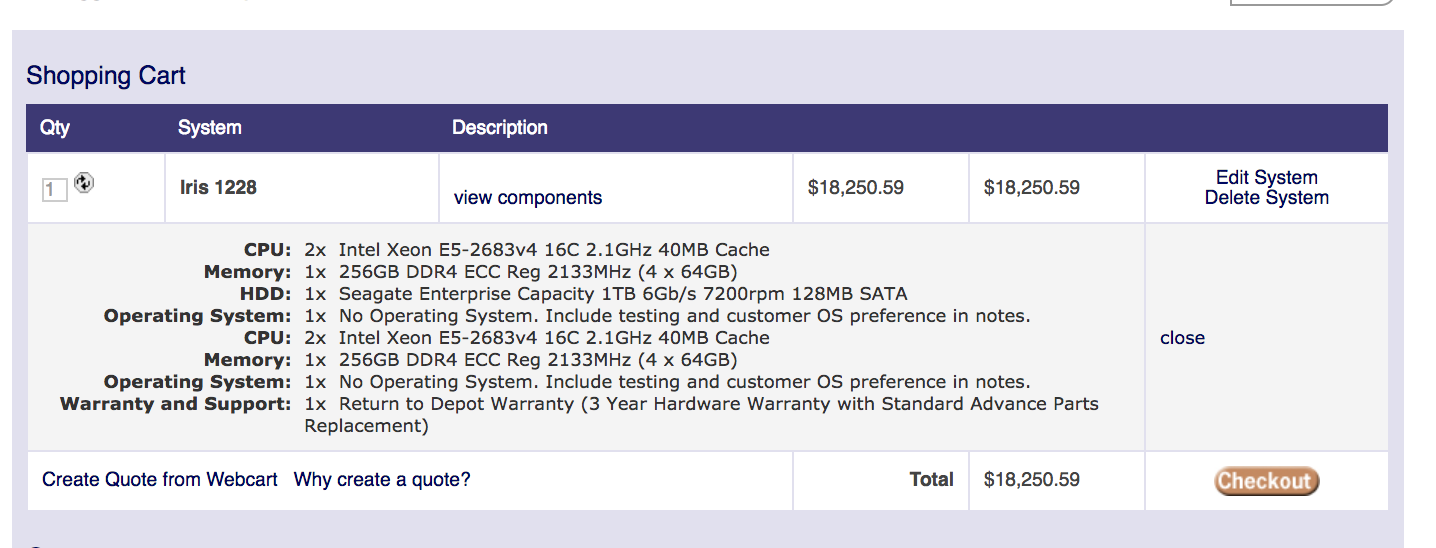
\includegraphics[scale=.6]{cpuConfig3}\\
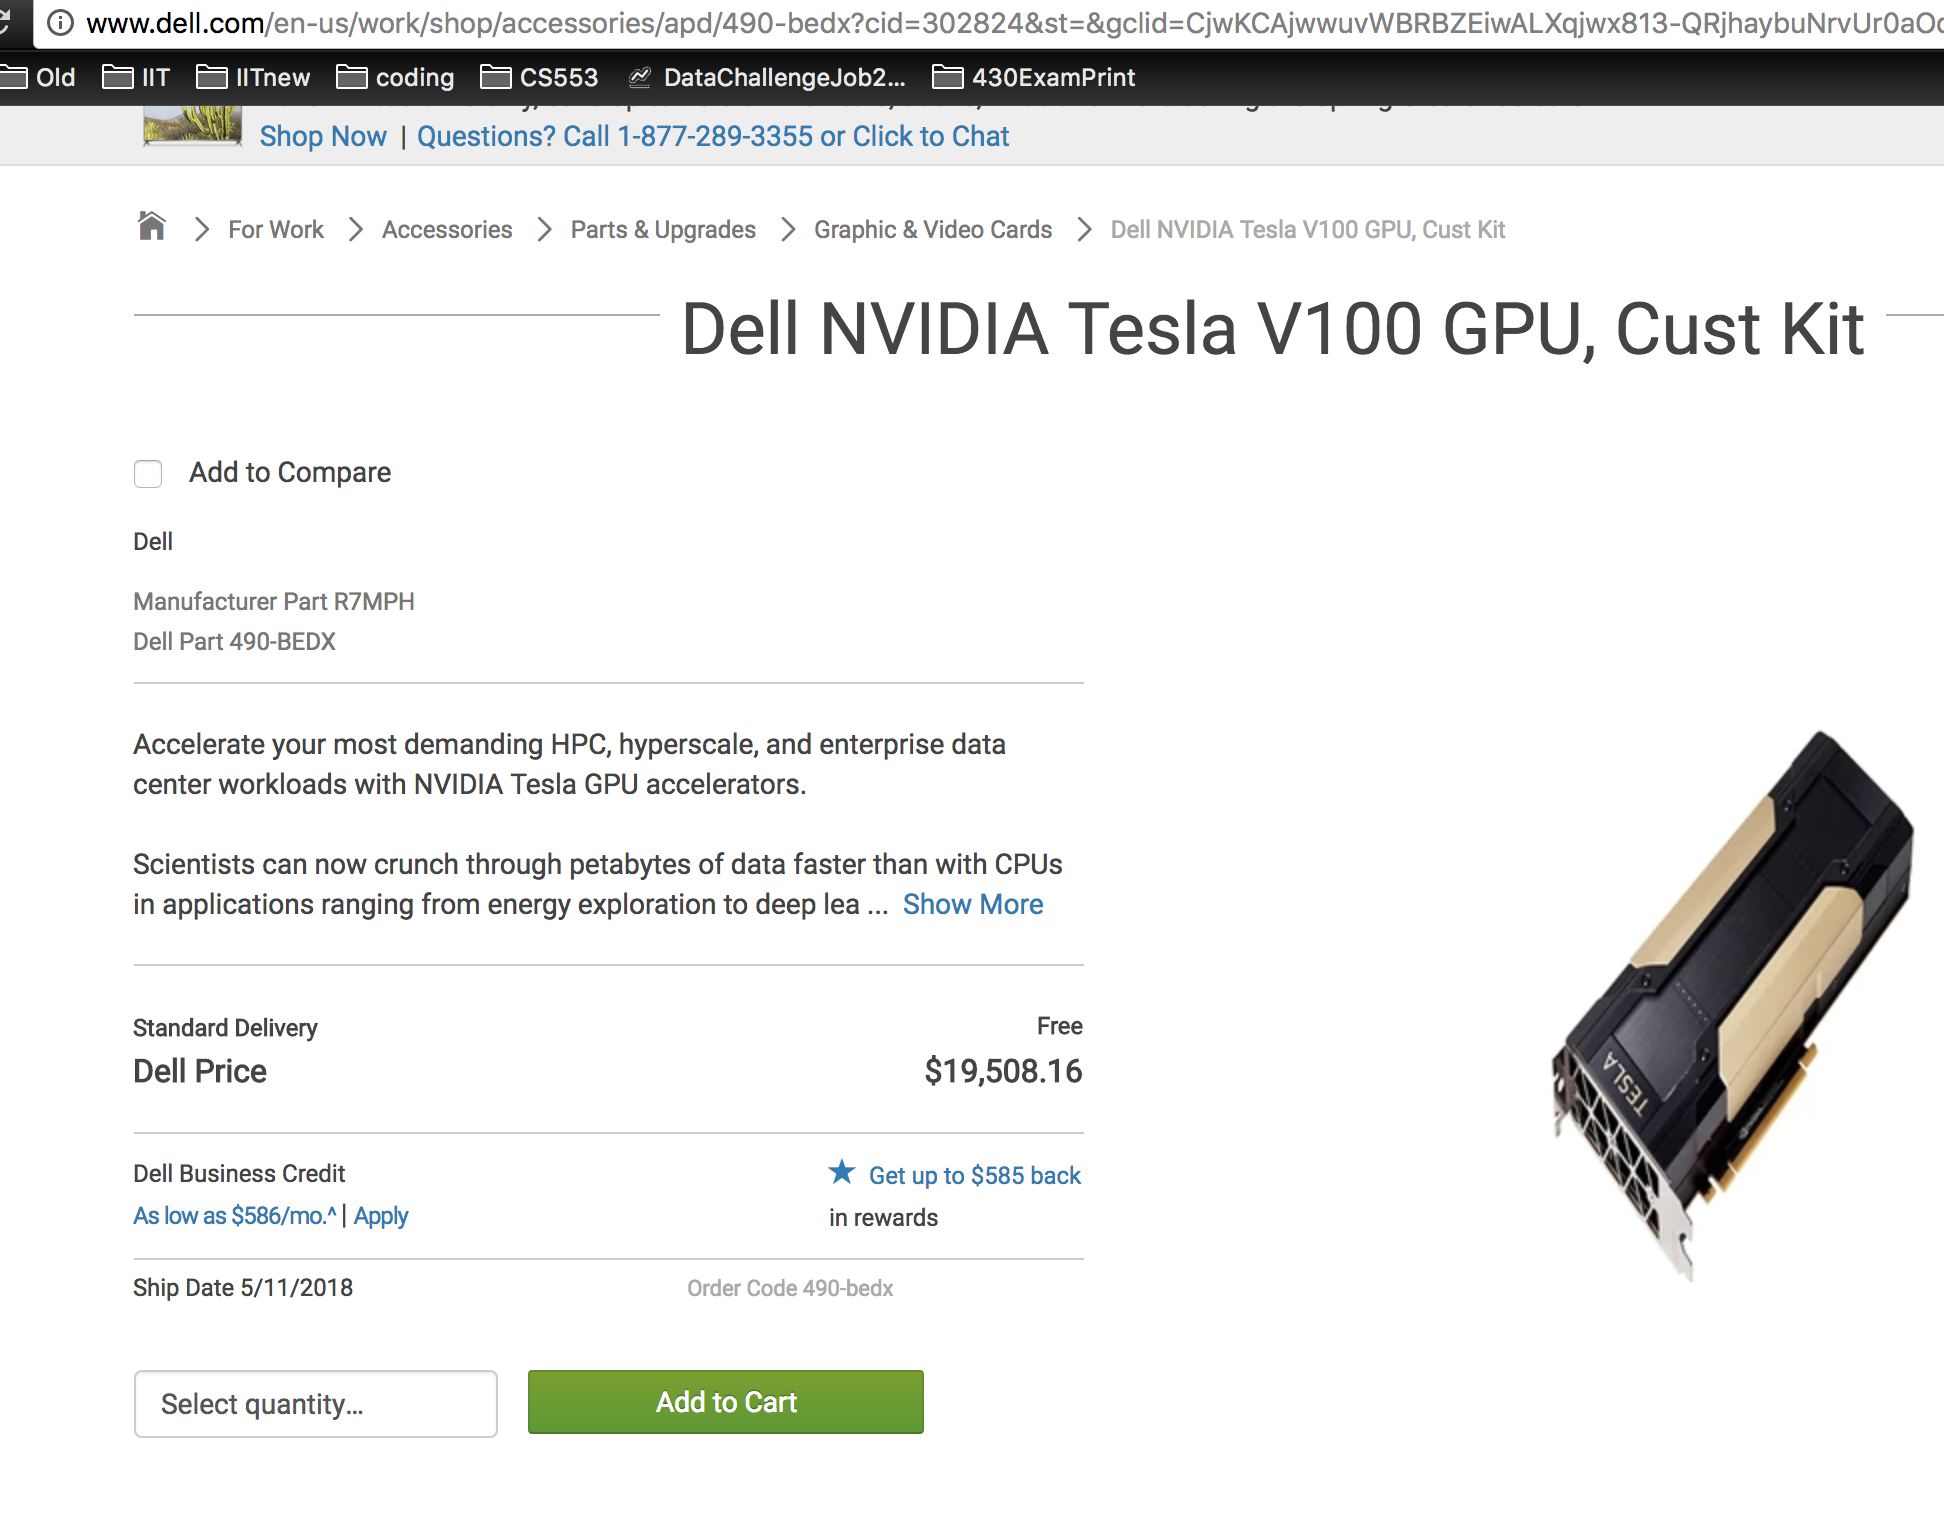
\includegraphics[scale=.3]{gpu}\\

\emph{Fat-Tree network Infiniband}\\
\\
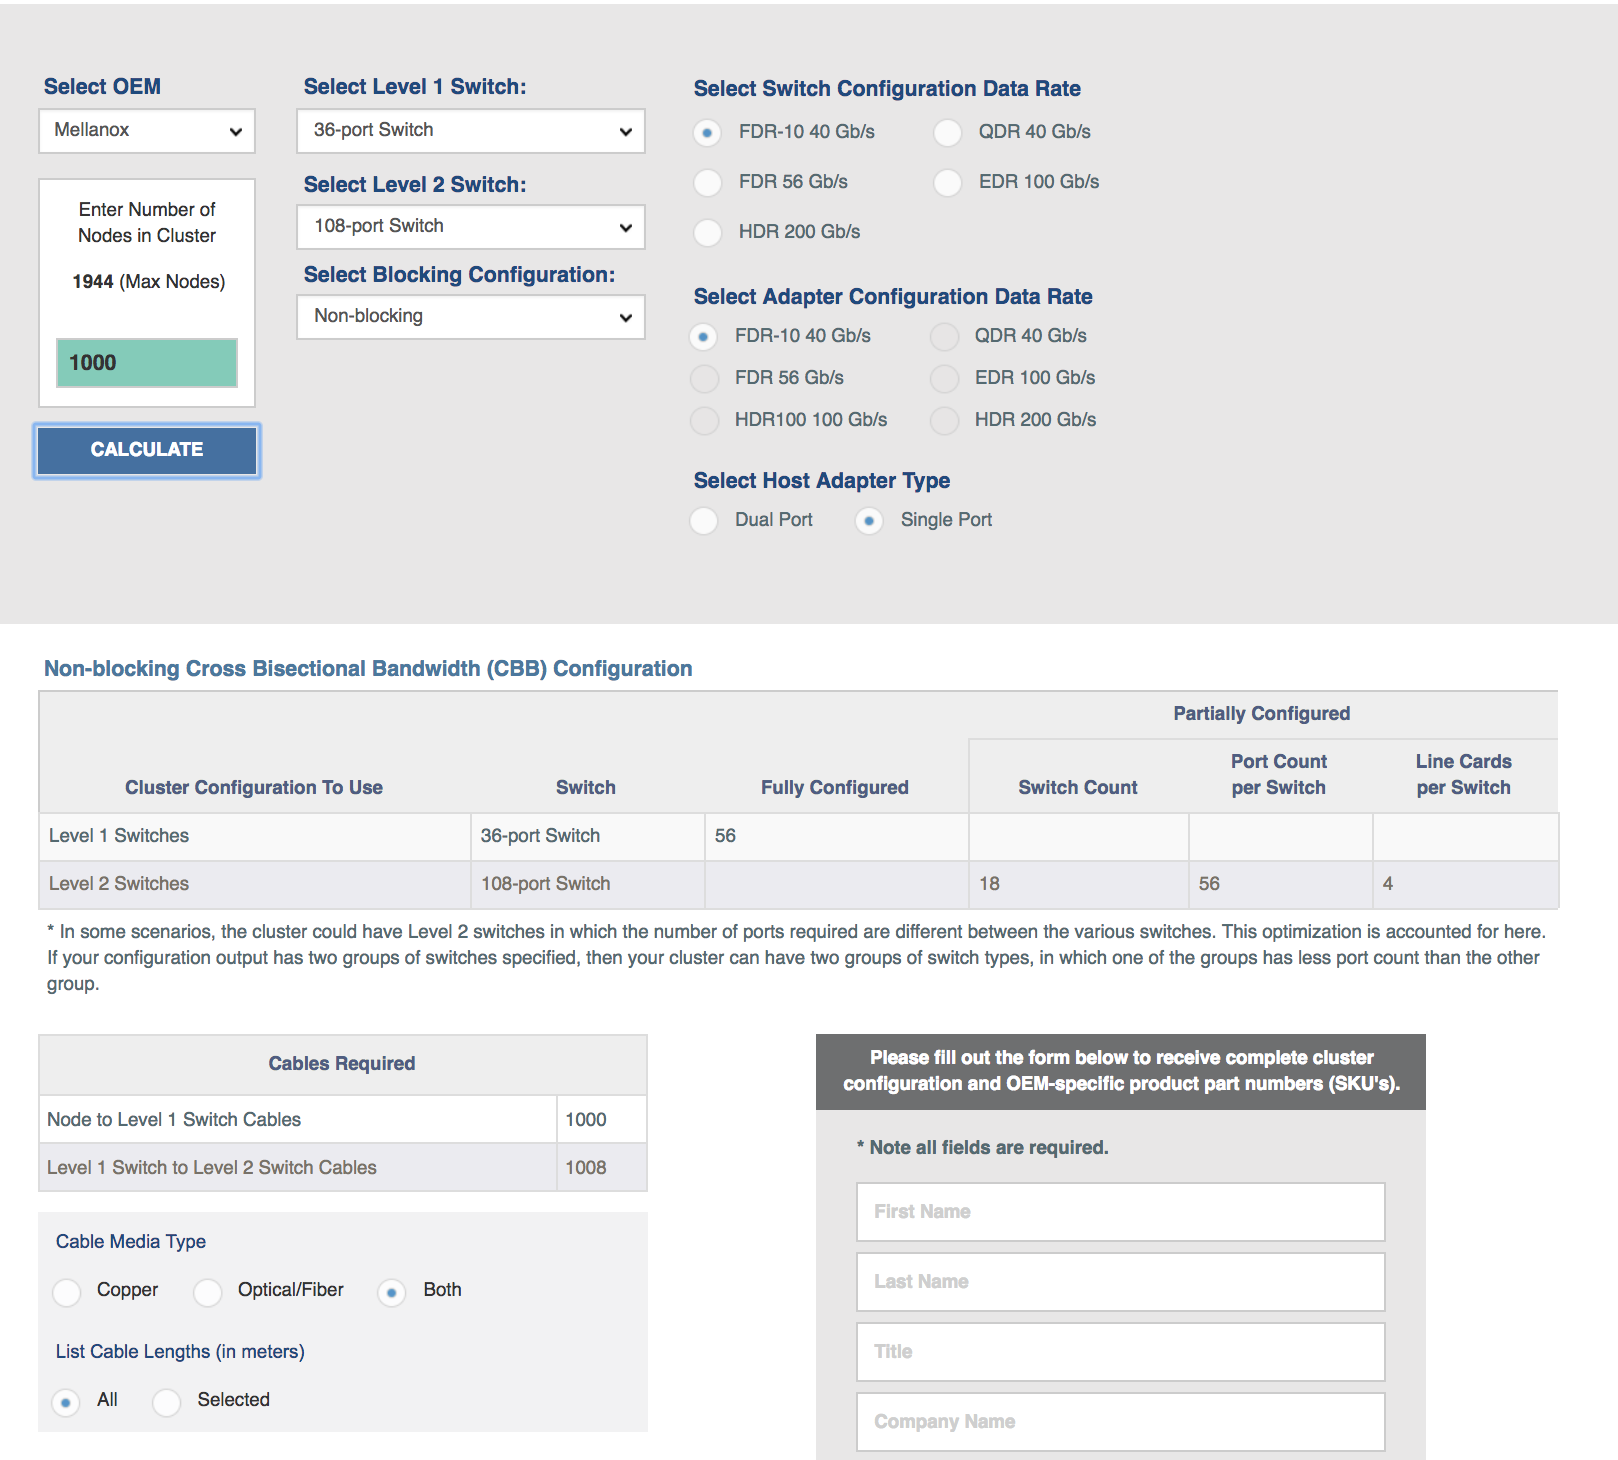
\includegraphics[scale=.4]{switchConfig3}\\

\emph{Power usage}\\
\\
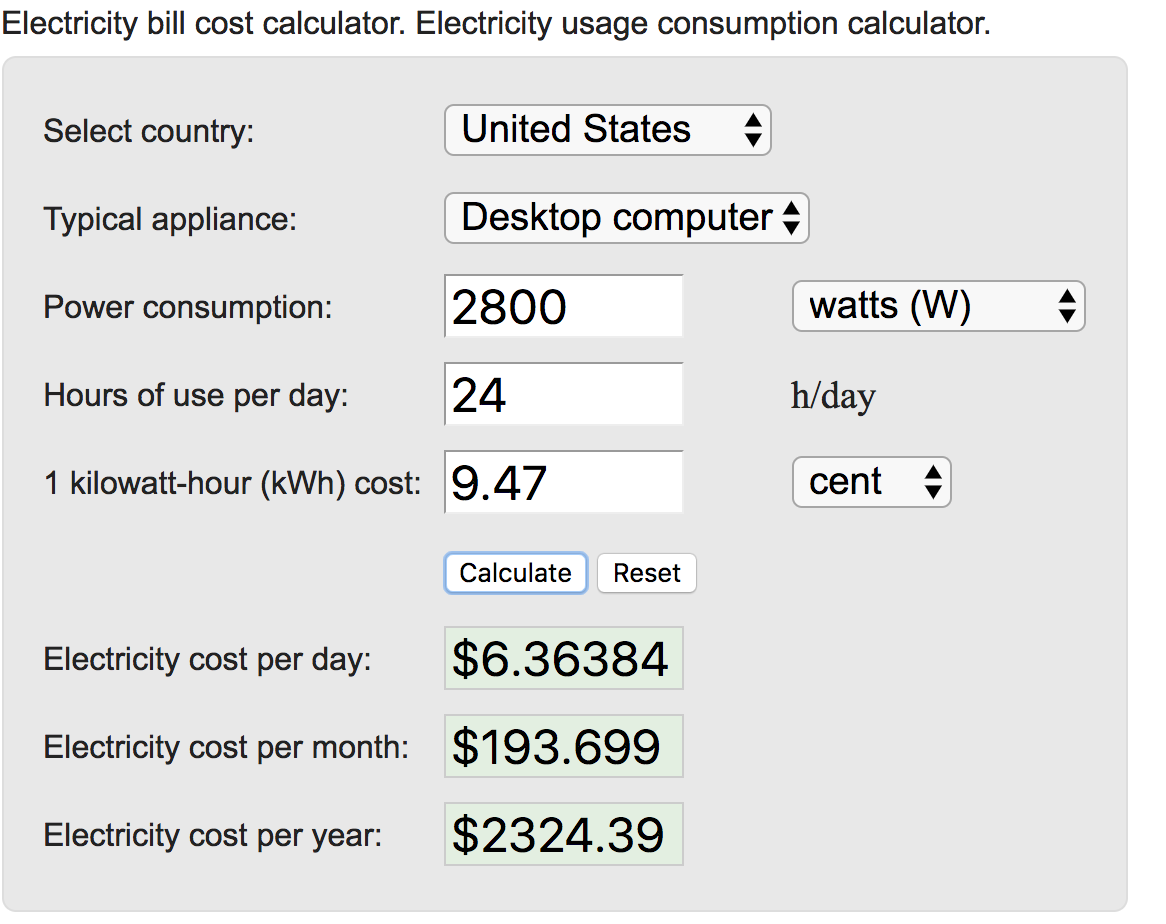
\includegraphics[scale=.3]{electricity3}\\

\textbf{\emph{Summary}}
\\
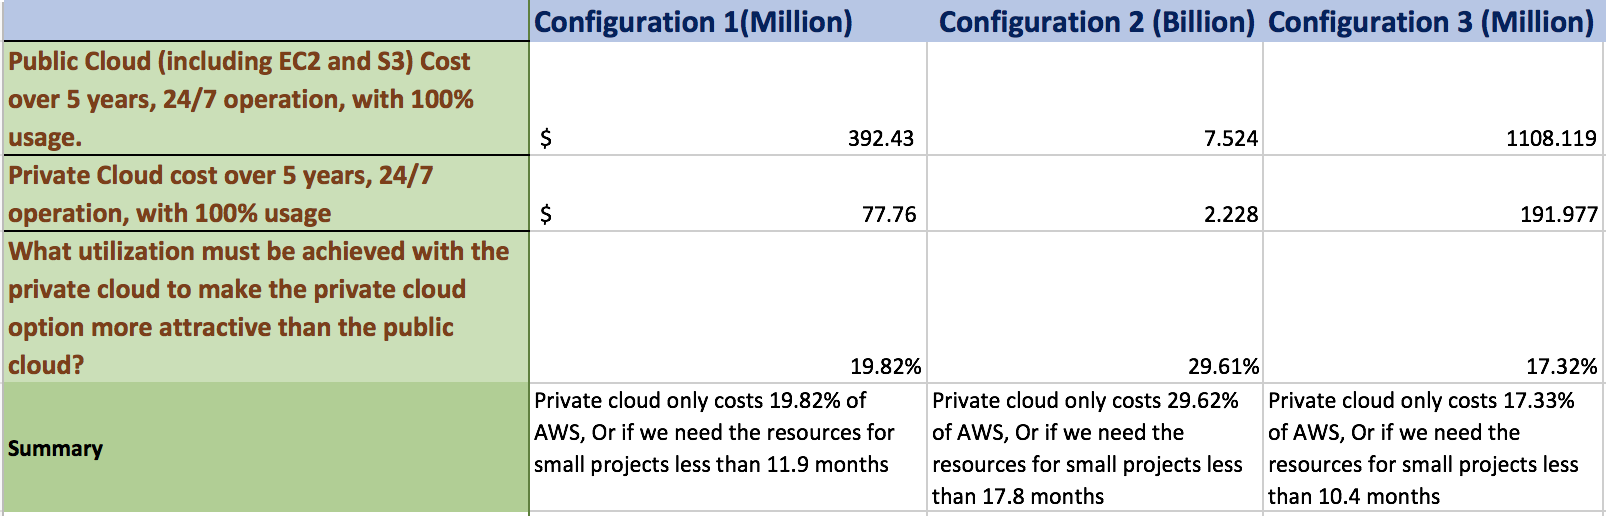
\includegraphics[scale=.6]{summary}\\



\end{document}